\documentclass{report}

\usepackage[margin=1in]{geometry}
\usepackage{tikz}

\usetikzlibrary{shapes,arrows}

\begin{document}

\title{SpLATS Lazy Automated Test System}


\section*{About}

This report explains the purpose and development of SpLATS Lazy Automated Test System (SpLATS), a tool used to automatically generate regression tests for Ruby.  Regression tests are tests that ensure that a program does not break any existing functionality when code is refactored, added to or patched. The aim of the project is to develop methods of automated testing in Ruby, to ultimately to reduce the amount of time Ruby developers spend writing tests and finding and fixing bugs. As Ruby is a fully-featured programming language a subset for SpLATS to use was defined, called Lightweight Ruby, so that the scope of the project was of reasonable size.




\section*{Technical Details}

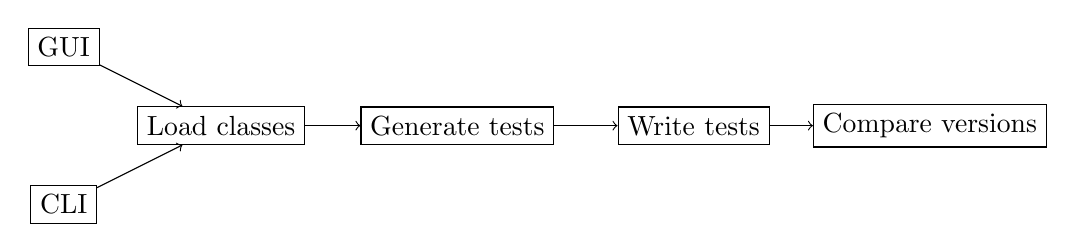
\begin{tikzpicture}
    \coordinate(origin);
    \node(core) at (origin) [draw] {Generate tests};
    \node(control) at ([left=3cm] core) [draw] {Load classes};
    \node(output) at ([right=3cm] core) [draw] {Write tests};
    \node(compare) at ([right=3cm] output) [draw] {Compare versions};
    \node(gui) at ([left=2cm,above=1cm] control) [draw] {GUI};
    \node(cli) at ([left=2cm,below=1cm] control) [draw] {CLI};

    \draw[->] (control) -> (core);
    \draw[->] (core) -> (output);
    \draw[->] (output) -> (compare);
    \draw[->] (gui) -> (control);
    \draw[->] (cli) -> (control);
  \end{tikzpicture}\\
{A simplified summary of the control flow of SpLATS} \\


\section*{Software Engineering}

The research-oriented nature of the project made it difficult to use agile methods as group methods often saw conflicting solutions to problems, and often it proved to be quicker for a single member to prototype code instead of explaining complex ideas.

Timetabling constraints were a recurring problem, there were few times where all group members were available.


The group first tried short, daily meetings, with longer meetings where possible or necessary.
    We quickly found that conflicting schedules made the short meetings impossible for all group members to attend and served little purpose: most days not enough progress was made to warrant discussion.
    Daily meetings are useful in the workplace where team members can meet everyday for considerable periods of time. They are not so possible when the group members between them do seven modules and two humanities options. Therefore, there were two hour-long meetings per week, where one was directly followed by a meeting with the project supervisor.

    After trying several online communication methods, we found a project IRC channel was helpful, hosted on EsperNet.
    Commit messages from Git were posted there, and it was especially useful for discussions during the winter holidays, when we couldn't be in the same physical location. The conversations are also automatically logged, so members who were not present in the chat room at the time could catch up.






We decided at the outset to use the git revision control system for various reasons:
      \begin{itemize}
      \item We had all used it in the past and were comfortable with it.
      \item It is a distributed revision control system, which grants additional flexibility compared to centralised systems, as it allows for such things as offline working and private branches.
      \item It works very well with Unix-like systems, such as Linux, which all but one of the group uses.
      \item Git handles complex merging extremely well, and when there is a merge conflict, it is very easy to sort manually.
      \end{itemize}

\section*{Conclusions}
 
On the whole, SpLATS has succeeded. All of the requirements and many of the extensions were fulfilled, and it has been demonstrated to work on several test cases. The predominant open problem is reducing the exponential growth of the search space so that a limit imposed on the complexity of each test could be relaxed. If this were possible then the tests would instantly become considerably more complex and useful for testing purposes.
The group members have learned about larger scale collaboration, including the need for regular check-ins, meetings, and direct supervision by a senior.
SpLATS has scope for future improvement, by implementing smarter feedback-driven traversal methods, and supporting more language features.

\end{document}

